
\section*{Definitions}

% %
% %CADA activida debeestar ligada
% a un deseo potencial
% 
% imnPGT you cando X and Y. To do X 
% 


\MT algorithm has been presented in our paper (cite), therefore we suggest you to read the paper first.


The program tracks MST or segments, therefore you can conduct your analysis in either of those two ways.

\vspace{-7\baselineskip}\footnotetext{If your are not familiar with graph theory you might find theses links useful: 

 \url{http://en.wikipedia.org/wiki/Minimum_spanning_tree}

 \url{http://en.wikipedia.org/wiki/Glossary_of_graph_theory}}
\vspace{7\baselineskip}




\section*{The program and its calculations}


If you use MST, the species' MST will be compared to all species MST, comparing each segment but outputing the answer by species, so you can expect at most nsp posible tracks, where nsp is the number of initial species.
	

\vspace{-7\baselineskip}\footnotetext{nsp = number of species}
\vspace{7\baselineskip}

If you use segments each segment will be compared to all species MST, comparing each segment and outputing the answer by segments/points, so you can expect at most nsegs, where nseg is
	
	sum MST(i)
		j=1 -$>$ nsp
		i=number of segments MST(j)
		    
		
As all segments or MST are not congruent, the real number of answers lies in a number smaller than those.



\subsection*{\MT files. General information}


The program uses two input files,



1. -the input file with the distributional data. (Only the input file is mandatory).
	
	
2. -the parameters/orders file with the values for parameters and the commands to be executed in bash 
	

	
and creates a kml output file


\subsection*{\MT input file}

\MT accepts as an input, a text file comprised of three columns,
	
	labels   lat   long
	

separated by tabs or spaces but not commas (,), most spreadsheet and sig programs can output shuch text files, or you can use awk/bash to reshape them. 


\label{valid_data_set}
\index{valid input data set}

\vspace{-7\baselineskip}\footnotetext{a valid data set = test0.dat

\begin{center} 
\begin{tabular}{lll}
sp1 & 1 & 9\\
sp1 & 3 & 11\\
sp1 & 6 & 12\\
sp2 & 1 & 9\\
sp2 & 1 & 10\\
sp2 & 3 & 10\\
sp2 & 4 & 11\\
sp2 & 5 & 12\\
sp2 & 6 & 12\\
sp3 & 4 & 13\\
sp3 & 5 & 11\\
sp3 & 8 & 8\\
sp4 & 4 & 12\\
sp4 & 6 & 11\\
sp4 & 7 & 8\\
sp5 & 8 & 8\\
sp5 & 7 & 6\\
sp5 & 8 & 2\\
sp6 & 8 & 8\\
sp6 & 7 & 5\\
sp6 & 8 & 3
\end{tabular}
% \caption{data from test0.dat}
 

\end{center}

}
\vspace{7\baselineskip}
	
As an example we include 

		-a bash+awk command file that converts a comma delimitated file in a \mt inputfile (csv2pt.sh)

		-a bash+awk command file that converts a GlobalMapper output in a \mt inputfile (gm2pt.sh)


\vspace{-7\baselineskip}\footnotetext{note: if your label field includes inner tabs/spaces, these will be considered as field separator therefore are NOT allowed, you can replace 
	such character by an underscore or delete them all (\mt converts the dash to underscore)}
\vspace{7\baselineskip}
		 
	 

\vspace{-7\baselineskip}\footnotetext{A common mistake is different labels for the same species, although \mt
	is not case sensitive, it is (quite) sensitive to mispellings therefore
	\cmd{Simulium} and \cmd{simulium} are the same, while \cmd{Simuliium}, \cmd{Simuliiun} or \cmd{Simuliun} are not.}
\vspace{7\baselineskip}
	
	
\subsection*{\mt output file}

\MT writes kml files, with or without the initial tracks. With all the analyses made before closing, in the form of tracks or points. The output is easily readable using google-earth or gis programs as QGIS. As some programs may or may not read the output, we only keep compatibility with google-earth/QGIS. If your beloved gis program does not read the output, please consider read it with google-earth.




\section{Download the program and a data set}
\index{download the program}
\label{download}

You must download a binary for your plataform of choice, from  \url{http://tux.uis.edu.co/labsist/martitracks} or \url{http://code.google.com/p/martitracks/}


Binaries are provided for Linux 64, Win 32 and 64


and the data sets at \url{http://tux.uis.edu.co/labsist/martitracks/data-example.zip}


\vspace{-7\baselineskip}\footnotetext{For linux version, you might need to convert the file \mt-xx to an execute file by typing in a command-line window:

 \framebox[2in][l] {\prompt \cmd{chmod +x \mt}}}
\vspace{7\baselineskip}


\section{Command modes}
\index{command modes}

\MT has two uses-interfaces: 1. A text user interface, and 2. a command-line interface. 


in the text user interface (TUI), the user can choice among different options including: changes of parameters for analysis, track a pair, groups or the whole data, find the index of congruence (IC) between pairs of tracks, or among sevaral tracks. print kml file, etc.
The command line interface was created for search strategies previously defined. The input file, output file and parameters files must be defined.

\vspace{-7\baselineskip}\footnotetext{\url{http://en.wikipedia.org/wiki/Text_user_interface\#TUI_under_Unix-like_systems}}
\vspace{7\baselineskip}

\subsection{Text user interface}

\index{tui:text user interface}

\label{openprogram}

You can use the text interface by simply typing at the promt: 

\framebox[2in][l] {\prompt \cmd{ ./{\mt} }}

for Linux, and 

\framebox[2in][l] {\prompt \cmd{ {\mt-winXX.exe} }}

for Windows in a command-line window 


or by clicking on the \MT icon (win. only).

 
\vspace{-7\baselineskip}\footnotetext{
TUI typography: commands will be  \tui{c}ut, to indicate that the instruction is cut and the letter to be pressed is c]}
\vspace{7\baselineskip}


\textbf{1. Enter the input name}: As soon as you open \mt, it asks for the input file name:

\begin{center}
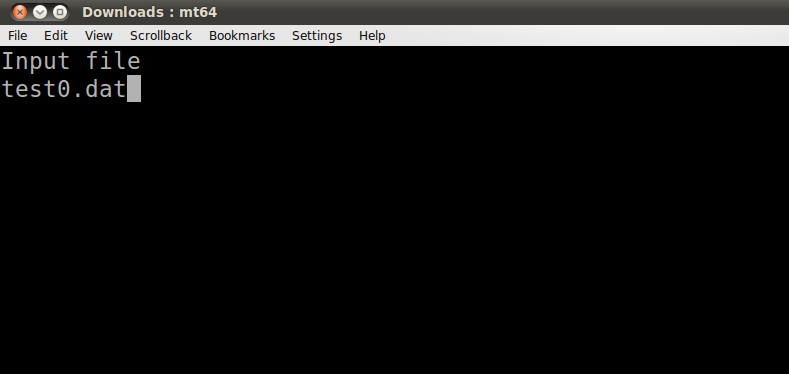
\includegraphics[scale=0.4]{./graphics/input-file.png}
 % input-file.png: 789x374 pixel, 72dpi, 27.83x13.19 cm, bb=0 0 789 374
\end{center}

\textbf{2. Set up the analysis:} Once you specified the input name, a list of commands help the users to set up the analysis.

\begin{center}
 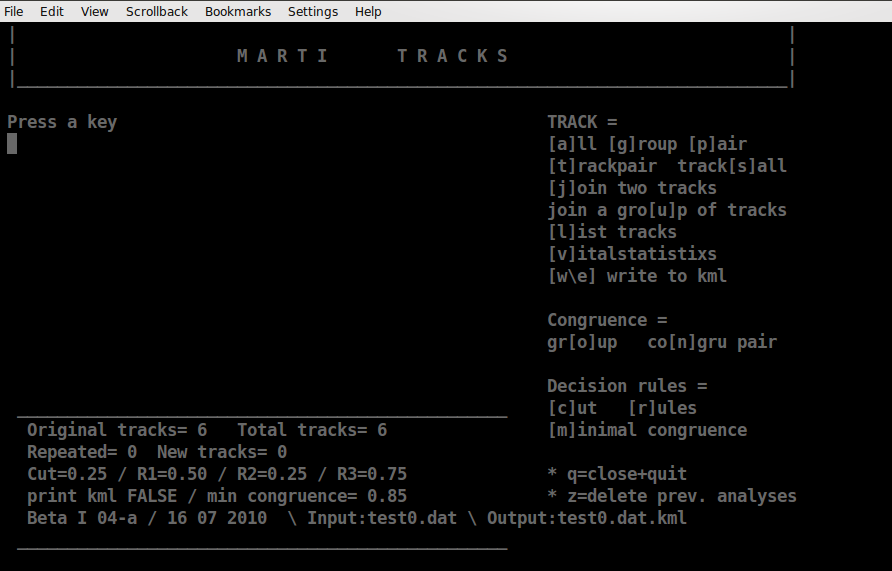
\includegraphics[scale=0.4]{./graphics/text-interface.png}
 % text-interface.png: 1237x678 pixel, 72dpi, 43.63x23.92 cm, bb=0 0 1237 678
\end{center}


Then we must define the values of the parameters, to be used in this analysis. 

There are five parameters: \tui{c}ut value, 

three \tui{r}ules of decision,  and the value for \tui{m}inimal congruence.

And we are ready to conduct our analysis. As we might have similar initial MSTs, we need to joint those MST that are the same according to the minimum value of \tui{m}inimal congruence fixed. We must press \tui{u}, to join the gro\tui{u}p. The program will ask thenumber of the initial and final track to be joint. Now we must use  \tui{a}ll, to find the congruent segments and define  the generalized tracks or distributional patterns of species. 

Finally, we need to eliminate those redundant generalized tracks, typing again \tui{u}, but joint from the track number 7  to the track 9, because first six tracks are individual tracks.

If, we want to write our results  in a kml file, we must type \tui{k} and \tui{+} to activate the output to the  kml file. The kml info must change from FALSE to TRUE. Then, we will use \tui{w} if we want to write the whole information of the analysis including: individual tracks, and generalized tracks, or we can type \tui{e} to write only the generalized tracks into the kml file.


For the command-line user interface we need to specified: the input file, output file, and parameters file.


\framebox[4.4in][l] {\prompt \cmd{ ./{\mt}-64 <input file> <output file> <parameters file>}}

